%% ----------------------------------------------------------------
%% Thesis.tex -- main
%% ---------------------------------------------------------------- 

\documentclass[a4paper, 10pt, oneside]{memoir}
%% Use the option citeauthor to be able to use citet. The default cite will still work.
\usepackage[citeauthor]{basilea}
\usepackage{listings}
\usepackage{lipsum}
\usepackage{caption}
\usepackage{makecell}
\usepackage{multirow}
\usepackage{placeins}
\usepackage{mathtools}
\usepackage{hyperref}
\usepackage{adjustbox}
\usepackage{diagbox}

\usepackage{stackengine}
\usepackage{rotating}
\usepackage{tabularx}

\newcounter{cons}[subsection]
\renewcommand{\thecons}{\roman{cons}}
\newcommand\consCount[1]{\refstepcounter{cons} \text{(#1-\roman{cons})}}

\newcounter{rownumber}[table]
\renewcommand{\therownumber}{\thefigure.\arabic{rownumber}}

\newcommand{\false}{$\textit{false}$}
\newcommand{\true}{$\textit{true}$}
\newcommand{\ocean}{\mathcal{O}}
\newcommand{\flood}{\digamma}
\newcommand{\walk}{\mathcal{W}}
\newcommand{\island}{\mathcal{I}}
\newcommand{\nb}{\mathcal{N}}
\newcommand{\pseudo}{\lstset%
{%
    emph=[1]%
    {%
        If,
        While,
        Else,
        For,
        AdderNetworkEncoder,
        BuildBDD,
        Return,
    },
    emphstyle=[1]{\bfseries},
    %
    emph=[2]% Variable Types
    {% 
       false,
       true,
    },
  emphstyle=[2]{\textit{}\ttfamily},
}}
\DeclareRobustCommand{\rchi}{{\mathpalette\irchi\relax}}
\newcommand{\irchi}[2]{\raisebox{\depth}{$#1\chi$}} %https://tex.stackexchange.com/questions/103885/how-to-type-an-inline-chi-in-latex

\lstdefinelanguage{Pseudo}{
    morekeywords={If, While, Else},
    sensitive=false, % keywords are not case-sensitive
    morecomment=[l]{//}, % l is for line comment
    morecomment=[s]{/*}{*/}, % s is for start and end delimiter
    morestring=[b]" % defines that strings are enclosed in double quotes
}



%% ----------------------------------------------------------------

\title				{Encoding Diverse Sudoku Variants as SAT Problems}
\thesistype			{Bachelor Thesis}

\department 		    {Department of Mathematics and Computer Science}
\faculty			{Natural Science Faculty of the University of Basel}
\research		    {Artifical Intelligence Research Group \\ \url{https://ai.dmi.unibas.ch/}}

\examiner    		{Prof. Dr. Malte Helmert}
\supervisor  		{Augusto B. Corrêa}

\authors     		{Sebastian Schlachter}
\email				{sebastian.schlachter@unibas.ch}
\immatriculnr		{2017-927-534}

\date				{20.07.2022}

% switch here for the german logo to logo-de
\ulogo				{Template/logo-en} 


%% ----------------------------------------------------------------
\begin{document}

% for english use \selectlanguage{english}, for german use \selectlanguage{ngerman}
\selectlanguage{english}

\thesisfront
\maketitle
\pagestyle{thesis}
%% ----------------------------------------------------------------
% !TEX root = ../Thesis.tex
\chapter{Acknowledgments}
I want to thank everyone who accompanied me during the writing of this thesis, especially my supervisor Augusto B. Corrêa, which always supported me with honest feedback and an open ear regarding questions or concerns. Further, I would like to sincerely thank Prof. Dr. Malte Helmert for giving me the opportunity to write this thesis on a subject that turned out to be incredibly engaging and joyful to work on.
%% ----------------------------------------------------------------
% !TEX root = ../Thesis.tex
\chapter{Abstract}
Sudoku has become one of the world's most popular logic puzzles, arousing interest in the general public and the science community. Although the rules of Sudoku may seem simple, they allow for nearly countless puzzle instances, some of which are very hard to solve. SAT-solvers have proven to be a suitable option to solve Sudokus automatically. However, they demand the puzzles to be encoded as logical formulae in Conjunctive Normal Form. In earlier work, such encodings have been successfully demonstrated for original Sudoku Puzzles. In this thesis, we will present encodings for rather unconventional Sudoku Variants, developed by the puzzle community to create even more challenging solving experiences. Further, we demonstrate how Pseudo Boolean Constraints can be utilized to encode Sudoku Variants that follow rules involving sums.

%% ----------------------------------------------------------------
\thesistoc
%% ----------------------------------------------------------------
%\thesisnomencl
%% ----------------------------------------------------------------
\thesismain
% !TEX root = ../Thesis.tex
\chapter{Introduction}

Sudoku Puzzles excite, as the rather simple task of filling out a grid with numbers becomes a demanding challenge just by stating a small set of rules that must be followed. For a $9 \times 9$ grid of cells which may already contain numbers, the original Sudoku rules every puzzle solver must follow are: A number with a value from 1 to 9 must be placed in each cell, and every number may appear only once per column, row and marked $3\times3$ box. An example of a normal Sudoku Puzzle and its solution is shown in Figures \ref{fig:SudokuManOfMystery} and \ref{fig:SudokuManOfMysterySolution}.

\begin{figure}
\vspace{2.5mm}
\centering
\begin{minipage}{.4\textwidth}
    \centering
    \captionsetup{justification=centering,margin=0cm}
    \includegraphics[width=.8\textwidth]{Figures/SudokuManOfMystery.png}
    \captionof{figure}{Normal Sudoku Puzzle \cite{CrackingTheCryptic2021}}
    \label{fig:SudokuManOfMystery}
\end{minipage}%
\begin{minipage}{.4\textwidth}
  \centering
    \captionsetup{justification=centering,margin=0cm}
    \includegraphics[width=.8\textwidth]{Figures/SudokuManOfMysterySolution.png}
    \captionof{figure}{Solution to Puzzle\\in Figure \ref{fig:SudokuManOfMystery}}
    \label{fig:SudokuManOfMysterySolution}
\end{minipage}
\end{figure}

Using these rules, the puzzle in its original form was first seen in the early 80s and established itself as one of the most popular logic puzzles in the last few decades. Since the mid-2000s, Sudokus also became an inherent part of the puzzle section in many newspapers and gained a fan community of puzzlers eager to develop and solve more challenging riddles. Around this time, researchers also started publishing first papers analysing Sudokus. For example, in 2006, it was shown by \cite{jarvis2006mathematics} that there are $6.671\times 10^{21}$ valid $9\times 9$ Sudoku grids. In the same year, Lynce and Ouaknine published a paper \cite{Lynce2006SudokuAsASATProblem} showing how Sudoku Puzzles can be encoded into logical formulas in a way that SAT-solvers can be used to find their solutions. SAT-solvers are suitable for solving Sudokus because most of the puzzles are “well-formed”, which means they only have one solution that is deducible without ambitions. Or, as \cite{Lynce2006SudokuAsASATProblem} states, ``Such puzzles are meant to be solved without search, i.e., merely with reasoning.''\\
\\
In this thesis, we aim to go one step further and find encoding methods for Sudoku Variants that are based on original Sudoku but augment the rules with additional requirements that solutions must fulfil. Our source of choice for such rather unconventional Sudoku Variants and rules will be the book ``Cracking The Cryptic Greatest Hits'' (\emph{CTCGH}) \cite{CrackingTheCryptic2021}, which presents a collection of the most unique, entertaining but also demanding Sudoku Variants the puzzle community came up with until today. The book was published after a successful Kickstarter campaign by Mark Goodliffe and Simon Anthon, which run one of the most famous Youtube channels focused on Sudokus: ``Cracking The Cryptic''\cite{ChannelCrackingTheCryptic}. In their videos, they present and solve puzzles sent to them from people all around the world, allowing them to create this phenomenal assortment of diverse Sudoku Variants.\\
\\
To get a foretaste of the variants we will work with, one may solve the Sudoku depicted in Figure \ref{fig:Thermo2020}. The normal Sudoku rules apply, but instead of already filled out cells, seven so-called \emph{Thermometers} are placed on the grid. For each thermometer, it must hold that starting from the bulb, the cell values along the thermometer can only strictly increase. As one will see, this already suffices to guarantee the uniqueness of the solution.\\
\\
As we intend to make the encodings of different rules compatible with each other, it will be possible to encode and solve new Sudoku Variants formed by arbitrarily combining said rules. To test our encodings, though, we will use puzzle instances from CTCGH and state of the art SAT-solvers like MiniSat. Comparing the encodings and the performance of the SAT-solvers working on them, we will show that for most puzzle instances from CTCGH, SAT-solvers can find a solution within seconds. However, we will also find exceptions to this, with Sudoku Variants that require extensive encodings and comparably high solving times by the SAT-solvers, revealing that the task of encoding and solving these special Sudoku Variants is by no means a trivial one.\\
\\
Because we will examine many Sudoku Variants with rules involving sums, we also want to further elaborate on the encoding of Pseudo-Boolean Constraints. Following the ideas of \cite{Een2006TranslatingPC}, we will show how Binary Decision Diagrams and Adder Networks can be used to encode Pseudo-Boolean Constraints and how the two methods compare to each other.

\begin{figure}
\centering
\captionsetup{justification=centering,margin=0cm}
\includegraphics[width=\textwidth]{Figures/Thermo2020.png}
\caption{Example of a Sudoku Puzzle using Thermometers,\\puzzle by Akash Doulani, CTCGH page 15 \cite{CrackingTheCryptic2021},\\this is a corrected version, available at \cite{OnlineSolutionThermo2020} }
\label{fig:Thermo2020}
\end{figure}






% !TEX root = ../Thesis.tex

\chapter{Background}
Before we dive into how we can translate Sudokus into a language such that a computer can work on them, we first elaborate on some background knowledge and definitions needed to understand the used tools and formalisms.

\section{Propositional Logic}
Propositional logic is a language that provides a formal way of writing statements that can either be true or false. It is used in this thesis to describe and encode the specific rules of the different Sudoku Variants. This section will shortly introduce the common syntax and semantics.

\paragraph{Atoms}
(also called \emph{atomic propositions}) are the smallest units used in propositional logic, and must have a truth value of true or false (often noted as digits 0 and 1).

\paragraph{Literals}
are atoms or their negation, so if $x_1$ is an atom, then $x_1$ and $\neg x_1$ are literals. Literals are said to be \emph{positive} or \emph{negative} respectively.


\paragraph{Formulas} are compositions of one or multiple atoms and can be defined recursively:\\
Every atom is also a formula.
If $\varphi$ is a formula, then so is its negation $\neg\varphi$.
If $\varphi$ and $\psi$ are formulas, then so is the conjunction $\varphi \land \psi$.
If $\varphi$ and $\psi$ are formulas, then so is the disjunction $\varphi \lor \psi$.


\paragraph{Interpretations} (also called truth assignments) are functions that assigns truth values to a set $A$ of atoms $\mathcal{I}: A \rightarrow \{0,1\}$. A formula $\varphi$ over $A$ holds (is true) under an interpretation $\mathcal{I}$ (written $\mathcal{I} \models \varphi$) following the semantical rules:
\begin{center}
    \begin{tabular}{ l l l }
    $\mathcal{I} \models x_1$ & iff & $\mathcal{I}(x_1) = 1$\\
    $\mathcal{I} \models \neg x_1$ & iff & not $\mathcal{I} \models x_1$\\
    $\mathcal{I} \models (\psi \land \varrho)$ & iff & $\mathcal{I} \models \psi$ and $\mathcal{I} \models \varrho$\\
    $\mathcal{I} \models (\psi \lor \varrho)$ & iff & $\mathcal{I} \models \psi$ or $\mathcal{I} \models \varrho$\\
\end{tabular}\\
Where $\psi$ and  $\varrho$ are formulas and $x_1$ is an atom.
\end{center}An interpretation for which a formula $\varphi$ hold is called a \emph{model} of $\varphi$.

\paragraph{Equivalence}
of two formulas $\varphi$ and $\psi$ is given if it holds for all interpretations $\mathcal{I}$ that, $\varphi$ holds under $\mathcal{I}$ if and only if $\psi$ holds under $\mathcal{I}$. The formulas are then called \emph {logically equivalent} ($\varphi \equiv \psi$).

\paragraph{Implications / Biconditionals}
As one might have noticed, implication ($\rightarrow$) and biconditional ($\leftrightarrow$) have not been mentioned in the definition of formulas as they are abbreviations for more extended formulas that use $\lor$, $\land$ and $\neg$.
\begin{center}
\begin{tabular}{ l l l }
    $(\varphi \rightarrow \psi)$ & $\equiv$ & $(\neg\varphi \lor \psi)$\\
    $(\varphi \leftrightarrow \psi)$ & $\equiv$ & $(\neg\varphi \lor \psi) \land (\neg\psi \lor \varphi)$\\
\end{tabular}
\end{center}

\paragraph{Clauses}
are disjunctions of literals (atoms and/or their negations). A formula that is a clause is true under interpretation $\mathcal{I}$ if one of its literals is true.

\paragraph{Conjunctive Normal Form (CNF)}
A formula is said to be in conjunctive normal form if it is a conjunction of clauses. 
For example, given the atoms \emph{a}, \emph{b}, \emph{c} and \emph{d}, the formulas $\varphi$, $\psi$ and $\varrho$ are in CNF:
\begin{center}
    \begin{tabular}{ l l l }
    $\varphi$ & $\equiv$ & $(a)$\\
    $\psi$ & $\equiv$ & $(a \land b)$\\
    $\varrho$ & $\equiv$ & $((a \lor b) \land (c \lor d))$\\
\end{tabular}
\end{center}
Also, it holds that every formula can be brought into CNF \cite{LogicForComputerScientists}, and a formula in CNF can be noted as a set of sets of literals, for example, $\varrho \equiv \{\{a,b\},\{c,d\}\}$.

\section{SAT-Problems and SAT-Solvers}
SAT-Problems (also called \emph{Satisfiability Problems} or \emph{Boolean Satisfiability Problems}) describe the problem of deciding if a formula of propositional logic is satisfiable (if there exists a model for it) or not. SAT-solvers are programs or algorithms that try to solve instances of this problem. They take a formula as input and return a boolean value (true or false) to indicate if a model exists or not. Most SAT-solvers also directly provide a model if they can find one. In the experiments of this thesis, multiple SAT-solvers are used, which are described in further detail in \ref{MiniSatAndSat4j}. As we will later see, the time to find solutions for particular problem instances varies between them. However, when it comes to computational complexity, it holds that SAT-Problems are in NP and that they are NP-Hard\cite{10.1145/800157.805047}\cite{levin1973universal}, so the runtime of the solvers may scale exponentially with the number of clauses and variables given to them as input.

\subsection{DIMACS CNF File Format}\label{DIMACS}
The used SAT-solvers require the input formula to be in CNF. Further, they expect them to be described in the DIMACS CNF File Format, often just called DIMACS. The abbreviation DIMACS stands for Center for ``Discrete Mathematics and Theoretical Computer Science", which is a collaboration between Rutgers and Princeton University and research firms. The file format was utilised in the DIMACS Implementation Challenge 1993 and since then has become the common file format for SAT-Problems.\\

DIMACS CNF Files have the following Format:
\begin{itemize}
    \item Atoms are represented as positive integers.
    \item Negative literals are represented as negative integers.
    \item The first line starts with the letter ``p" and holds the problem description. It states the problem type, the highest integer used to describe an atom and the number of clauses.
    \item Clauses are represented as lists of their literals and are terminated by the number 0. White spaces or line breaks separate all literals and the ending 0s.
    \item Lines are interpreted as comments (ignored by the solver) if they start with the letter ``c". Comments can be added everywhere in the file except inside the definition of a clause.
\end{itemize}
A DIMACS file describing the formula $\varphi \equiv (x_1 \lor \neg x_2) \land (x_2 \lor x_3) \land (\neg x_1 \lor \neg x_3) \land (\neg x_1 \lor \neg x_2 \lor x_3)$ could look like this:

\lstset{basicstyle=\ttfamily}
\begin{lstlisting}[language=Java,frame=single]
c some comment describing the problem
p cnf 3 4
 1 -2  0
 2  3  0
-1 -3  0
-1 -2  3  0
\end{lstlisting}


\subsection{How SAT-Solvers solve}
Given a formula, a SAT-solver must decide if it is satisfiable or not (We assume the formula is in CNF so it can be handled as a set of clauses). To do so, the solver tries to find a model by assigning truth values to atoms one by one. In a standard SAT-solver, this is not done randomly but by using the inference mechanism of \emph{unit propagation}. 
A famous algorithm using this mechanism is the DPLL algorithm \cite{DavisAMachineProgramForTheoremProving1962} which can be directly implemented into a SAT-solver.
DPLL applies three rules:
\begin{enumerate}
    \item If a clause contains only one literal (or multiple literals, but only one is still unbound and all the others do not make the clause true),  the value that makes the literal true must be assigned. Otherwise, the clause and the formula would become false. If a value gets assigned, all clauses containing the corresponding true literal can be removed from the set of clauses. The corresponding false literals can be removed from all remaining clauses since they can not make them true.
    \item If there is a literal that only appears in one polarity in all clauses (consistently positive/negative), its atom value can also be assigned to make the literals true.
    \item  If the set of clauses becomes empty, the formula is ``satisfiable". If an empty clause is derived, the formula is ``unsatisfiable". If no further assignments can be inferred and no decision can be made about satisfiability yet, a literal gets chosen. The algorithm would then continue in two branches, one where the chosen literal gets set to be true and one where it is set to be false. The formula is then satisfiable if and only if it is satisfiable under one of the two assumptions. Repeating this procedure of assigning values creates a Search-Tree of exponential size.
\end{enumerate}
SAT-solvers can strongly differentiate in how they choose the next atom to assign a value to and how they learn from entering unsatisfiable branches in the search tree.



\subsection{MiniSat and Sat4j}\label{MiniSatAndSat4j}
MiniSat is a lightweight SAT-solver that is based on ``the ideas for conflict-driven backtracking, together with watched literals and dynamic variable ordering" as the original paper \cite{EenAnExtensibleSAT-solver2004} states. Its original source code in C++ used less than 600 lines. The solver was further refined up to its current version 2.2, but for the experiments in this thesis we use version 1.4 for which precompiled binaries can be found at \cite{webMiniSat}.

Sat4j is a Java library that provides a SAT-solver that can be directly called and run in Java. It does not provide the best performance, but because it is easy to use and integrate, it is well suited for early experimenting and testing. The used version is 2.3.4. The library itself and further details can be found at \cite{webSat4j}.

MiniSat+ (a particular version of MiniSat) and Sat4j provide native support for Pseudo-Boolean Constraints. However, this feature will not be used because this thesis aims to translate Sudoku Puzzles into a form that can be solved with arbitrary SAT-solvers.

\section{Constraint Networks (CN)}
Puzzles like Sudoku can be broken down into multiple constraints that must all hold for a solution to be correct. Problems like this can be described using constraint networks. The issue of finding a solution to a constraint network is called Constraint Satisfaction Problem or short CSP. Solutions for constraint networks can be found using Backtracking Search (\cite{ArtificialAModernApproach}, page 175).However, this thesis aims to find such solutions by first encoding the Constraints into SAT-Problems that arbitrary SAT-solvers can then solve. This section will shortly discuss how constraint networks are defined and how they can be translated directly to general SAT-Problems.


Constraint Networks can be described as a tuple of three components: $CN := \langle \mathcal{X},  \mathcal{D},  \mathcal{C}\rangle$.
$\mathcal{X}$ is a set of variables, $\mathcal{D}$ is a set of finite domains (one corresponding to each variable), and $\mathcal{C}$ is a set of constraints that describe the allowed values for variable subsets.

\subsection{Unary Constraints}
Constraints that only consider one variable are called unary constraints. They do not have to be explicitly written as part of $\mathcal{C}$ because they can also be seen as a domain restriction for a variable that can be represented by reducing the corresponding domain. Examples for a variable $x_1$ could be: ``$x_1$ must be smaller than 10", ``$x_1$ must be larger than 0", or ``$x_1$ must be even".

\subsection{Binary Constraints}
Constraints that include two variables are called binary constraints. They get defined extensively as part of $\mathcal{C}$ by listing all allowed value pairs that the two variables could take. Examples for CSP variables $x_1$ and $x_2$ could be: ``$x_1$ must be smaller than $x_2$", ``$x_1$ or $x_2$ must be 9", or ``$x_1 + x_2 \leq 12$".

\subsection{N-ary Constraints}
Constraints that include more than two variables are called N-nary constraints and get defined similarly to binary constraints in a CSP. Examples for variables $x_1$ to $x_9$ could be: ``At most one CSP variable from $x_1$ to $x_9$ may be 5" or ``The sum of the CSP variables $x_1$ to $x_9$ must be 45".

\subsection{Common Encodings}
There are many different ways to transform a CSP into a set of clauses that a SAT-solver can work on, two of the most common ones we want to elaborate on here.

\paragraph{Direct Encoding \cite{walsh2000SATvCSP}\cite{gent20002ArcConsistencyInSAT}}
We assign a SAT variable $x_{i,j}$ to all possible variable values $j$ for all CSP variables $i$. \emph{At-least-one} clauses ensure that a CSP variable i has at least one out of the $d$ values assigned from its domain.
\begin{center}
    $x_{i,1} \lor x_{i,2} \lor ... \lor x_{i,d}$
\end{center}

\emph{At-most-one} clauses ensure that a CSP variable $i$ has at most one value assigned from its domain.
\begin{center}
    $\neg x_{i,j} \lor \neg x_{i,k}$\\
    $\forall x_{i,j}, x_{i,k} \in D_i$ s.t. $j\neq k$ 
\end{center}

\emph{Conflict} clauses ensure that no CSP variable value combinations are allowed that do not comply with the CSP's constraints.
For example, The N-ary constraint ``at most one CSP variable of $x_1$, $x_2$ and $x_3$ has value 5" would be transformed into the following conjunction of clauses:
\begin{center}
 $(\neg x_{1,5} \lor \neg x_{2,5}) \land (\neg x_{1,5} \lor \neg x_{3,5}) \land (\neg x_{2,5} \lor \neg x_{3,5})$. 
\end{center}

Assuming the CSP has $n$ variables that have a domain of size $d_i$, the transformation would in total lead to $n$ at-least-one clauses and per variable to $\sum_{m=1}^{d_i} (m-1)$ at-most-one clauses. For the constraints, however, we can only give an upper bound for the number of needed clauses per constraint equal to the product of the domain sizes of the contained variables.

\paragraph{Support Encoding \cite{kasif1990OnTheParallelComplexityOfDiscreteRelaxationInConstraintSatisfactionNetworks}\cite{gent20002ArcConsistencyInSAT}}
The same at-least-one and at-most-one clauses are used as in the direct encoding, but instead of conflict clauses, we add so-called support clauses. For all pairs of variables $x_i$ and $x_j$ in a constraint, we add a clause for all domain values of $x_j$. These clauses define the allowed values of the other variables of the constraint.However, not all these clauses must be necessary. They can be left away if the CSP variable value corresponding to $x_{j,d}$ is allowed with all values of CSP variable $x_i$. 
This is best shown in an example, assume all CSP variables have a domain of \{1, 2, 3, 4, 5\}, the N-ary constraint ``at most one CSP variable of $x_1$, $x_2$ and $x_3$ has value 5” could then be transformed to the clauses:
\begin{center}
 $\neg x_{1,5} \lor x_{2,1} \lor x_{2,2} \lor x_{2,3} \lor x_{2,4}$\\
 $\neg x_{2,5} \lor x_{1,1} \lor x_{1,2} \lor x_{1,3} \lor x_{1,4}$\\
 $\neg x_{1,5} \lor x_{3,1} \lor x_{3,2} \lor x_{3,3} \lor x_{3,4}$\\
 $\neg x_{3,5} \lor x_{1,1} \lor x_{1,2} \lor x_{1,3} \lor x_{1,4}$\\
 $\neg x_{2,5} \lor x_{3,1} \lor x_{3,2} \lor x_{3,3} \lor x_{3,4}$\\
 $\neg x_{3,5} \lor x_{2,1} \lor x_{2,2} \lor x_{2,3} \lor x_{2,4}$\\
\end{center}
In this case further clauses like $\neg x_{1,1} \lor x_{2,1} \lor x_{2,2} \lor x_{2,3} \lor x_{2,4} \lor x_{2,5}$ can be added, but they are redundant because if the CSP variable $x_1$ takes the value 1 the constraint does allow all possible values for $x_2$. Generally, the support encoding requires more clauses than the direct encoding, but this does not make it inferior or necessarily slower for SAT-solvers \cite{gent20002ArcConsistencyInSAT}. 


\subsection{Pseudo-Boolean Constraints (PBCs)}
Constraints that describe equations like $w_1x_1+w_2x_2+...+w_nx_n \leq K$ are called Pseudo-Boolean Constraints. The variables $x_1$ to $x_n$ have boolean domains, the $w_i$s are called weights, and K is called bound (or RHS). Both the weights and the bound must have integer values. If a variable $x_i$ gets assigned a truth value of true/false, it gets valued 1/0 in the equation. PBCs can be transformed into clauses by first converting them to Binary Decision Diagrams (BDD), Adder Networks or Sorter Networks. Within this thesis, we will use the former two variants following the ideas of \cite{Een2006TranslatingPC}, which we will elaborate on further in section \ref{encoding:PBCs}.

\section{Sudoku}\label{NormalSudoku}
The family of logic puzzles called Sudoku is based on the Latin Squares Problem. In its current form, it was first published in the US in 1979 by Howard Garns as ``Number Place". In 1984 the puzzle became popular in Japan,  where it got the name ``Sudoku" (translated: ``digit-single") which is the name under which it later became famous around the world.
A \emph{normal} Sudoku Puzzle consists of a $9\times9$ grid, partially already filled with numbers from 1 to 9 named clues. Additionally, the grid is divided into smaller sub-areas called boxes, consisting of  $3\times3$ cells. To solve the puzzle, one has to assign a value from 1 to 9 to each free cell so that each number is present in each row, column, and box.\\
For most Sudoku instances, there is the additional property that they only have one solution. There must be at least 17 clues for this to hold, as \citet{doi:10.1080/10586458.2013.870056} show. An example of a Normal Sudoku Puzzle can be seen in Figure \ref{fig:exampleSudoku}. For a more accessible annotation, we define a coordinate system on the Sudoku grid, which can be seen in Figure \ref{fig:GridCoordinates}. With this coordinate system, a grid cell can be specified using a tuple of two numbers $(x,y)$ which is how we reference specific cells from now on. Countless variations and rules can be added to the original Sudoku Puzzle to create new (and eventually harder) solving experiences. The book ``Cracking The Cryptic Greatest Hits" \cite{CrackingTheCryptic2021} contains an extensive collection of Sudoku Variants, a few of which are introduced in the next chapter (\ref{SudokuVariantsAndRules}) and further elaborated during this thesis.

\begin{figure}
\centering
\includegraphics[width=0.5\textwidth]{Figures/17-clue sudoku puzzle (McGuire).png}
\caption{Example of a Sudoku Puzzle with 17 clues by \citet{doi:10.1080/10586458.2013.870056}.}
\label{fig:exampleSudoku}
\end{figure}

\begin{figure}
\centering
\includegraphics[width=0.5\textwidth]{Figures/GridCoordinates.png}
\caption{Coordinate system for grid cells.}
\label{fig:GridCoordinates}
\end{figure}


% !TEX root = ../Thesis.tex
\chapter{Sudoku Variants and Rules}\label{SudokuVariantsAndRules}
This chapter introduces the most common Sudoku variants and rules used in CTCGH \cite{CrackingTheCryptic2021}, which are all based on the normal Sudoku rules introduced in Section \ref{NormalSudoku}. Meaning the normal Sudoku rules still apply, in addition to the rules of the variants introduced in this chapter. The aim here is to give an overview, so the descriptions are on a high level and relatively informal. All A formal definition and further details on how the constraints and types are encoded to CNF can be found in chapter \ref{Encoding}.

\section{Killer Sudoku}
In a Killer Sudoku, the normal Sudoku rules apply. Additionally, some (not necessarily all) orthogonally adjacent cells are grouped in so-called cages. Each cell can be part of at most one cage. For each cage, two constraints must hold, firstly, the values of all its cells must have a certain sum (\emph{target sum}), and within a cage, each value may only appear once. The cages are often marked on the grid with dashed lines or by colouring their cells, and a small number is placed in the top-left cell of a cage to specify its targeted sum. See Figure \ref{fig:exampleKiller} for an example.

\begin{figure}
\centering
\includegraphics[width=0.6\textwidth]{Figures/Killer Example (CTC page 36).png}
\caption{Section of a Killer Sudoku showing 4 cages, from CTCGH \cite{CrackingTheCryptic2021} page 36.}
\label{fig:exampleKiller}
\end{figure}

\section{Thermometers}
Thermometers placed on the Sudoku grid connect multiple adjacent cells sequentially (without branching). Each thermometer has a bulb cell marked with a filled circle, and its other cells are marked with a line outgoing from this circle. For a thermometer, it must hold that starting from the bulb, the cell values along the thermometer can only strictly increase. CTCGH \cite{CrackingTheCryptic2021} also contains a version called ``Frozen Thermometers" that allows cell values along a thermometer to stay the same. Additionally, it differs from puzzle to puzzle instance, whether thermometers are allowed to overlap each other or not.

Thermometers are also part of the unique puzzle on page 52 of CTCGH \cite{CrackingTheCryptic2021}. In this puzzle, only three hint digits and the shape and orientation of 8 thermometers are given. It is then up to the solver to deduce the position of the thermometers, which can not overlap.\todoMissing{Figure}

\section{Sandwich Sums}
Sandwich Sums are constraints that can be applied to rows, columns or cages. They require certain cells to have a particular sum, which is specified for each row and column at the grid's edge or inside an affected cage. To fulfil a Sandwich Sum Constraint, it must hold that the sum of all cells lying between the cells containing the values 1 and 9 is equal to the specified target sum. The cells containing 1 and 9 are not included in the sum. Example: a row containing the numbers [2, 4, 8, 9, 6, 5, 1, 7, 9] has a Sandwich Sum of 6 + 5 = 11. CTCGH \cite{CrackingTheCryptic2021} also includes a variation ``Sandwich Sums - 1 to X", where a target sum must be hit, but the second value that defines the sums border is not defined and must be deduced to a value of 2 to 9.\todoMissing{Figure}

\section{Secret Direction}
The Secret Direction constraints is used in a unique Sudoku Puzzle described on page 41 of CTCGH \cite{CrackingTheCryptic2021}. Following an adventure's backstory to find a buried treasure, the constraint requires a solution with a ``secret path" from a shaded starting cell to the only cell with value 9, which is also the centre of a 3x3 box. The hidden path must be reconstructed in the following way, starting with the shaded cell; the current cell's value describes the length of the next step, and the position of the 9 in the current 3x3 box defines the direction. Once a step in the path is found, one must apply the same rules to find the next one until the treasure is discovered.

\section{Arrowheads}
Arrowheads placed on the Sudoku grid specify the partial or total order that must be respected between two adjacent cell values.

\section{Chess Moves}
Some Sudoku Variants use constraints named after chess figures to describe the relationship between two different cells. In CTCGH \cite{CrackingTheCryptic2021}, three of these constraints are introduced, which share the idea that if another cell can be reached from a cell by one chess move of a particular chess figure, these cells may not have the same value. The three constraints differ in the chess figure they use, as listed below.
\begin{itemize}
    \item Anti-Knight: Cells that are one knight move away from each other may not contain the same value. A knight move consists either of one or two steps in one direction on the current column or row followed by either one or two steps in the then-current row or column. In total, the length must be three steps, and a column and row must be used.
    \item Anti-King: Cells that are one king move away from each other may not contain the same value. The set of cells that are one king move away from a cell is equal to the set of cells that are directly orthogonally and diagonally adjacent to it.
    \item Anti-Queen: Cells that are one queen move away from each other may not contain the same value. Cells that are one queen move away from a cell are the cells that lie on the same row, column or diagonal as a cell.
\end{itemize}

\section{Towers}
The name Towers is used for a unique constraint in the puzzle on page 49 of CTCGH \cite{CrackingTheCryptic2021}. A tower describes a group of cells which is always based at the lowest row (nr. 9) and rises to a certain height. The different towers are marked by the differently shaded cells. Furthermore, below each tower at the grid's edge stands a number representing its target sum. There are two types of towers, normal and faulty ones. In a normal tower, the cell values are strictly increasing starting from the base and adding all its cell values together results in the target sum. Differently, the numbers are not strictly increasing, or the sums do not match in a faulty tower, but not both at once. As an additional help, it is stated how many towers have non-increasing values and for how many towers the sums will not match. However, it is then up to the solver to deduce which towers belong to which type.
% !TEX root = ../Thesis.tex
\chapter{Encoding}\label{Encoding}
As introduced in \ref{DIMACS}, the SAT-Solvers expect a DIMACS file as input that describes a set of clauses. This chapter details how the different Sudoku Variants and their rules can be encoded into these clause sets. We elaborate on the different variants separately, but as long as there are no direct contradictions, the different variants and rules could be freely combined (which can be done by creating the union of the corresponding clause sets). In the following formulae, we use the notation $s_{x_{n},...,x_{0}}$ to describe boolean variables, the corresponding integer numbers in the DIMACS files have the values $x_{n}*10^{n}+...+x_{0}*10^{0}$. For example, the literal $\neg s_{1,2,3}$ would be transformed to $-123$. There are two ways how we choose the name (number) for a variable during the encoding process:

\begin{enumerate}
    \item We use increasing values starting from 1. These dynamically chosen values are, by example, used for variables necessary to encode PBCs. We use $s_{v}$, for $v \in \mathbb{N}$, to describe them in the formulae as we do not know the corresponding integers in advance.
    \item  We use fixed intervals of numbers to encode certain constraints. Here every digit of a number has a semantic meaning. The dynamically generated variables skip these fixed intervals. For example, a fixed interval is used for the boolean variables that describe the cell values of the Sudoku grid. The variable $s_{x,y,z}$ is true if and only if cell ($x$,$y$) has the value $z$ assigned (as proposed in \cite{Lynce2006SudokuAsASATProblem}). The other used fixed intervals are indicated in the corresponding subsections of this chapter\todo{Actually do that!}. 
\end{enumerate}

It is important to note that the numbers used as variable names are not ``continuous". There are ``gaps". For example, not all integers from 1 to 1000 are used. This is because the dynamic variables skip the entire interval from 111 to 999, and the fixed variables used to encode cell values will not use numbers like 400 because we start to count rows at 1, and the grid cells can only hold values from 1 to 9. The needed fixed intervals grow larger when encoding more complicated variants, and with them often also the ``gaps". These gaps have no effect logically, but they can have a non-negligible effect on the time needed by the solvers, which is affected by the highest integer value used to describe a variable. However, as the ``gaps" are the same when encoding Sudokus with the same rules, they should not make a difference when comparing solver-times.

\section{Encoding of PBCs using Binary Decision Diagrams}\label{PBCEncodingBDD}
A binary decision diagram (BDD) is a directed graph that can be used to represent logical formulae. Every graph node corresponds to a partial assignment to the variables in the formula. The BDD has a root node which corresponds to the empty assignment. Every edge from a node $u$ to a node $v$ corresponds to an extension of the assignment of node $u$. Every node has at most two successors, one reachable via the edge that corresponds to assigning $true$ and one via the edge that corresponds to assigning $false$ to the next variable. Nodes store references to their successors as \emph{$true_{child}$} and \emph{$false_{child}$} respectively. Variables are considered in a fixed order. As recommended in \cite{Een2006TranslatingPC}, ordering them by decreasing\todo{do that} weight values is generally reasonable. If the variable value assignment determines the value of the entire logical formula that the BDD represents, the corresponding successor is a terminal node. Terminal nodes have no successors, as their corresponding assignment already satisfies the  logical formula, or it is impossible to extend the  assignment to satisfy the formula (The assignment of terminal nodes does not have to be a total one).\\

Since we want to encode PBCs, it is helpful to store for each node the sum that is achieved by adding together all the weights of the variables assigned to $true$ by the (partial) assignment of the node. Also, we assign an integer number to each node which can later be used to describe a boolean variable (called \emph{assignmentVariable}) that is true if and only if the partial assignment of the node is present.\todo{``present" is not correct...formulate it better...} \\

The BDD can be built using a Breadth-First-Search starting in the root, shown as pseudocode in \ref{CodeBDDConstruction}. The version we use for encoding PBCs differs from the one introduced in \cite{Een2006TranslatingPC} because it is written to encode equations rather than inequations. Further, the used queue has additional functionalities: Given a node, it can check if it already contains a node with the same attribute values and can return said equal node. The \emph{updated sums} of successor nodes either are the same as their predecessors ($false$ was assigned) or are equal to the sum of their predecessor plus the weight value corresponding to the edge that led to them (true was assigned).



{
\lstset%
{%
    emph=[1]%
    {%
        If,
        While,
        Else,
    },
    emphstyle=[1]{\bfseries},
    %
    emph=[2]% Variable Types
    {% 
       false,
       true,
    },
  emphstyle=[2]{\textit{}\ttfamily},
}
\begin{lstlisting}[frame=single,caption={Pseudo Code of BDD construction},captionpos=b, label=CodeBDDConstruction]
queue.append(root)
While not queue is empty:
    Node current = queue.poll()
    If assigning next variable leads to a total assignment:
        Node cT = Create true successor node with updated sum
        Node cF = Create true successor node with updated sum
    Else:
        Node cT = Create true successor node with updated sum
        If cT.sum >= RHS:
            # true successor is a terminal node
        Else:
            # true successor is not a terminal node
            If cT not in queue:
                queue.append(cT)
            Else:
                cT = queue.get(cT)
        Node cF = Create false successor node with updated sum
        If cF.sum + sum of remaining weights < RHS:
            # false successor is a terminal node
        Else:
            # false successor is not a terminal node
            If cF not in queue:
                queue.append(cF)
            Else:
                cF = queue.get(cF)
    current.true_child = cT
    current.false_child = cF
\end{lstlisting}
}

Once the BDD is built, we can transform it into clauses. In \cite{Een2006TranslatingPC}, it is explained how this can be achieved by treating the BDD network as a circuit of ITEs (if-then-else gates). However, it suffices to know that the BDD can be transformed by doing a second Breadth-First-Search starting from the root and that for each visited node that is not a terminal node, the following six implications must be added to the set of formulas:

\begin{enumerate}
    \item If the \emph{assignmentVariable} of the current node is true and the variable corresponding to the leaving edges from this node is true, then it follows that the \emph{assignmentVariable} of the $true_{child}$ node is true.
    \item If the \emph{assignmentVariable} of the current node is true and the variable corresponding to the leaving edges from this node is false, then it follows that the \emph{assignmentVariable} of the $false_{child}$ node is true.
    \item If the \emph{assignmentVariable} of the current node is false and the variable corresponding to the leaving edges from this node is true, then it follows that the \emph{assignmentVariable} of the $true_{child}$ node is false.
    \item If the \emph{assignmentVariable} of the current node is false and the variable corresponding to the leaving edges from this node is false, then it follows that the \emph{assignmentVariable} of the $false_{child}$ node is false.
    \item If the \emph{assignmentVariable} of the $true_{child}$ node is true and the \emph{assignmentVariable} of the $false_{child}$ node is true, then it follows that the \emph{assignmentVariable} of the current node is true.
    \item If the \emph{assignmentVariable} of the $true_{child}$ node is false and the \emph{assignmentVariable} of the $false_{child}$ node is false, then it follows that \emph{assignmentVariable} of the current node is false.
\end{enumerate}

Additionally, we add a clause that only contains the positive literal corresponding to the \emph{assignmentVariable} of the root node. Also, when visiting a node during this second Breadth-First-Search, we only append its children that are not terminal nodes. For children that are terminal nodes, we add a clause to the set of clauses: 
\begin{itemize}
    \item If the child's sum is equal to the RHS, a clause containing a positive literal corresponding to the \emph{assignmentVariable} of the child is added.
    \item If the child's sum is unequal the RHS, a clause containing a negative literal corresponding to the \emph{assignmentVariable} of the child is added.
\end{itemize}
An example is shown in Figure \ref{fig:BDDExample} where the BDD and the clauses are depicted that are used to encode the PBC $6*v_1+4*v_2+2*v_3=6$. The already achieved sums are written inside the nodes and the nodes \emph{assignmentVariables} are denoted as $a_i$ for $i\in \{1,2,3,4,5,6,7\}$. Edges with a circle are assigning $false$. Edges with a line are assigning $true$.

\begin{figure}
\centering
\includegraphics[width=\textwidth]{Figures/BDDExampleComposition.png}
\caption{BDD and clauses to encode $6*v_1+4*v_2+2*v_3=6$}
\label{fig:BDDExample}
\end{figure}


\section{Encoding of PBCs using Adder-Networks}\label{PBCEncodingAdderNetworks}

\section{Encoding of Sudoku Variants and Constraints}

\subsection{Normal Sudoku}
The normal Sudoku rules as introduced in \ref{NormalSudoku} can be broken down into the following five constraints, which can be encoded into clauses. The following encoding can be seen as a direct encoding using at-least-one and at-most-one clauses and was proposed by \cite{Lynce2006SudokuAsASATProblem} where it is called the minimal encoding:\\


\begin{table}[h!]
    \centering
    \begin{tabular*}{\textwidth}{l @{\extracolsep{\fill}}  c  c}
        \hline
        \\
        Constraint & Formula & \#Clauses\\
        \\
        \hline
        \\
        At least one number from 1 to 9 appears in each grid cell. & (S-\ref{S-i}) & 81\\
        \\
        Every number appears at most once per row. & (S-\ref{S-ii}) & 2916\\
        \\
        Every number appears at most once per column. & (S-\ref{S-iii}) & 2916\\
        \\
        Every number appears at most once per box. & (S-\ref{S-iv}) and (S-\ref{S-v}) & 2916\\
        \\
        Every cell that contains a hint can only have that value. & (S-\ref{S-vi}) & 1/hint\\
        \\
        \hline
    \end{tabular*}
        \caption{Constraints of Normal Sudoku.}
    \label{tab:NormalSudoku}
\end{table}


Formulae of clauses:\todo{Are "And" operators needed in last formula?}\\
\begin{tabular*}{\textwidth}{ l @{\extracolsep{\fill}} c}
    \\
    $\displaystyle \bigwedge_{x=1}^9 \bigwedge_{y=1}^9 \bigvee_{z=1}^9 s_{x,y,z}$  & \consCount{S} \label{S-\roman{cons}}\\
    \\
    $\displaystyle \bigwedge_{y=1}^9 \bigwedge_{z=1}^9 \bigwedge_{x=1}^9 \bigwedge_{i=x+1}^9 \neg s_{x,y,z} \lor \neg s_{i,y,z}$  & \consCount{S} \label{S-\roman{cons}}\\
    \\
    $\displaystyle \bigwedge_{z=1}^9 \bigwedge_{x=1}^9 \bigwedge_{y=1}^9 \bigwedge_{i=y+1}^9 \neg s_{x,y,z} \lor \neg s_{x,i,z}$  & \consCount{S} \label{S-\roman{cons}}\\
    \\
    $\displaystyle \bigwedge_{z=1}^9 \bigwedge_{i=0}^2 \bigwedge_{j=0}^2 \bigwedge_{x=1}^3 \bigwedge_{y=1}^3 \bigwedge_{k=y+1}^3 \neg s_{(3*i+x),(3*j+y),z} \lor \neg s_{(3*i+x),(3*j+k),z}$  & \consCount{S} \label{S-\roman{cons}}\\
    \\
    $\displaystyle \bigwedge_{z=1}^9 \bigwedge_{i=0}^2 \bigwedge_{j=0}^2 \bigwedge_{x=1}^3 \bigwedge_{y=1}^3 \bigwedge_{k=x+1}^3 \bigwedge_{l=1}^3 \neg s_{(3*i+x),(3*j+y),z} \lor \neg s_{(3*i+k),(3*j+l),z}$  & \consCount{S} \label{S-\roman{cons}}\\
    \\
    $s_{x,y,input_{x,y}}$,  for every $(x,y)$ s.t. input$_{x,y}$ $\neq 0$  & \consCount{S} \label{S-\roman{cons}}\\
\end{tabular*}\\

    
\subsection{Anti-Knight}
To encode the Anti-Knight rule, one must ensure that for each grid cell (x,y), it is forbidden to have the same value as its neighbours. The term neighbour of a cell (x,y) here corresponds to the cells that are one knight distance away from it. The set of neighbours to cell (x,y) can be defined as:\\ $N(x,y) = \{(i,j)~|\texttt{ cell }(i,j) \texttt{ one knight distance from cell }(x,y)\}$.
\begin{table}[h!]
    \centering
    \begin{tabular*}{\textwidth}{l @{\extracolsep{\fill}} c  c}
        \hline
        \\
        Constraint & Formula & \#Clauses\\
        \\
        \hline
        \\
        \makecell[cl]{Cells that are one knight-distance apart (neighbours) \\ must have different values.} & (AK-\ref{AK-i}) & 2016\\
        \\
        \hline
    \end{tabular*}
        \caption{Constraints of Anti-Knight rule.}
    \label{tab:AntiKnight}
\end{table}


Formula of clauses:\\
\begin{tabular*}{\textwidth}{ l @{\extracolsep{\fill}} c}
    $\displaystyle \bigwedge_{x=1}^9 \bigwedge_{y=1}^9 \bigwedge_{(i,j)\in N(x,y)} \bigwedge_{z=1}^9 \neg s_{x,y,z} \lor \neg s_{i,j,z}$ &\consCount{AK} \label{AK-\roman{cons}}\\\
\end{tabular*}\\

\newpage
\subsection{Killer}
\paragraph{Using PBCs:} For every killer cage of the input, we create a list of its cells. From every list, a PBC is created as follows: For every cell (x,y) of a cage, we add $\sum_{i=1}^{9} (s_{x,y,i}*i)$ to the left-hand side of the PBC. The right-hand side of the PBC is set to the target sum that was given as input. The different PBCs (one for every killer cage) can then be encoded into clauses, as explained in \ref{PBCEncodingBDD} and \ref{PBCEncodingAdderNetworks}.

\paragraph{Using PBCs + Combinations:}
The PBC approach can be further optimized, because given a fixed number of summands not all values from 1 to 9 can be used to achieve a certain sum. In example if a cage has a target sum of 8 and consists of three cells, the number of possible value combinations to achive the target sum is fairly limited. There are only two possible value combinations $1+2+5=8$ and $1+3+4=8$, so the allowed values that the cells could take are 1, 2, 3, 4 and 5. When constructing the PBC this knowladge can be used to reduce the number of variable-value products on the left hand side of the equation. For every cell in a cage we only add the variable times the corresponding value (to the left hand side) if the value is an allowed one.

\paragraph{Using Combinations:}
Another possibility is to completely abandon PBCs and exploit that only certain value combinations are possible given a cage with a fixed target sum and fixed number of cells that belong to it. To encode this every combination is given a corresponding variable $varNum$ which is true iff the corresponding combination is used in a certain cage. This can then be encoded in the following way:\\

\begin{table}[h!]
    \centering
    \begin{tabular*}{\textwidth}{l @{\extracolsep{\fill}} c}
        \hline
        \\
        Constraint & Formula\\
        \\
        \hline
        \\
        \makecell[cl]{For every Cage $g$ and possible combination $c$ (for that \\
        cage) it holds that, either the cage's target sum is not \\
        achieved using combination $c$ or every cage cell \\
        contains at least one value of the combination.} & (K-\ref{K-i})\\
        \\
        In every Cage $g$ at least one combination $c_a$ is used. & (K-\ref{K-ii})\\
        \\
        In every Cage $g$ at most one combination $c_a$ is used. & (K-\ref{K-iii})\\
        \\
        \makecell[cl]{Every value from 1 to 9 appears at most once within \\
        the cells of a cage.} & (K-\ref{K-iv})\\
        \\
        \hline
    \end{tabular*}
        \caption{Constraints of Killer Sudoku rules.}
    \label{tab:Killer}
\end{table}

\newpage
Formulae of clauses:\\
\begin{tabular*}{\textwidth}{ l c @{\extracolsep{\fill}} c}
    \\
    $\displaystyle \bigwedge_{g:groups} \bigwedge_{c:combis_g} \bigwedge_{[x,y]:g} -s_v \lor \bigvee_{z:c}  s_{x,y,z}$ & & \consCount{K} \label{K-\roman{cons}}\\
    \\
    $\displaystyle \bigwedge_{g:cages} \bigvee_{a=1}^{\#combis_g} varNum_{a}$ & & \consCount{K} \label{K-\roman{cons}}\\
    \\
    $\displaystyle \bigwedge_{g:cages} \bigwedge_{a=1}^{\#combis_g} \bigwedge_{b=a+1}^{\#combis_g} \neg varNum_a \lor \neg varNum_b$  & & \consCount{K} \label{K-\roman{cons}}\\
    \\
    $\displaystyle \bigwedge_{g:cages} \bigwedge_{[x_i,y_i]:g} \bigwedge_{[x_j,y_j]:g} \bigwedge_{z=1}^{9} \neg x_i y_i z \lor \neg x_j y_j z$ & with $[x_i,y_i] \neq [x_j,y_j]$ &\consCount{K} \label{K-\roman{cons}}\\
\end{tabular*}\\


% !TEX root = ../Thesis.tex
\chapter{Experiments}
This chapter elaborates on how the different encodings perform and how the different Sudoku Variants compare.
The program to encode the various  puzzle instances is written in Java. We also use Java to call the different Solvers (introduced in \ref{MiniSatAndSat4j}) and to log the resulting data. All experiments are run on a personal computer using Windows 10. The PC has an AMD Ryzen 7 5800X 8-Core Processor (3.80 GHz) and 32 GB of RAM (from which the Java Virtual Machine (JVM) is allowed to use 28GB).\\

The configurations we test for each puzzle instance differ by: 
\begin{itemize}
    \item The used Solver: Sat4j or MiniSat
    \item The used PBC-Encoding: Binary Decision Diagrams or Adder Networks
    \item The used optimization level: what is encoded as PBC (only for Killer Sudoku)
\end{itemize}

Conducting runtime experiments on a personal computer using Java comes with the caveat that the reported times all include some noise because their executions may be affected by other processes running in the background or by JVM events like garbage collections. To mediate that, we run 60 instances for every experiment configuration and report the average runtime and corresponding standard deviations.\\

\newpage
\section{Disclaimer}
Early testing showed that the solving times depend heavily on the order in which clauses and literals are given to the solvers. This is critical because we store clauses in sets and treat them as sets themselves. So the order of clauses (and literals) is not strictly defined and can vary from run to run. To still obtain comparable results, we order the clauses by length and the literals by the absolute values that encode them. We arbitrarily decided to pass the clauses containing the most literals first and to sort the literals within a clause by increasing absolute values. Like this, the solvers get the same encoding as input if a problem is encoded and solved multiple times. However, eliminating this additional noise comes at the cost of having to sort all the clauses after they are created.\\
\\
Because we use a relatively small test set of different puzzle instances, it is important to note that assumptions made based on insights from the conducted experiments may not be applied to a general case. The reason for the limited size of the test set is that in the case of puzzles from CTCGH, they are very exotic and often unique. For Killer Sudokus Puzzles, many instances can be found, but writing the puzzle down into a format that the program can work on is very time-consuming as it has to be done manually.

\section{CTCGH Sudoku Variants compared using Sat4j and MiniSat}
Tables \ref{Experimnet:CTCGHMiniSatAdderNetworks} and \ref{Experimnet:CTCGHSat4jAdderNetworks} show the  outcome of encoding and solving thirteen different Sudoku instances with Sat4j and MiniSat, respectively. For puzzles where PBCs were needed, Adder Networks were used to encode them. The shown puzzle instances are from CTCGH and combine different variants and rules. An overview of which rules are present in each instance is given in Table \todoMissing{Rule Table}.\\

Studying the two tables, one can see that the solving times using MiniSat are significantly higher than the ones of Sat4j. This may have to do with the fact that the Sat4j library and its functions can be accessed directly by the Java program, whereas the MiniSat-Solver is called as an external executable. For all further experiments, we are only using Sat4j (which internally also contains a version of MiniSat). There is one exception to Sat4j always being faster. ``The Original Sandwich'' seems to perform much better with MiniSat, which we have no explanation for, but could, of course, also be the case for other instances we did not test.\\

Comparing the times needed for encoding to the ones needed for solving (using Sat4j), it turns out that for instances without PBCs, the encoding times are all higher than the solving times, which does not hold if PBCs are involved, where it differs from instance to instance which part takes longer.

\section{Adder Networks vs. Binary Decision Diagrams}
To analyze the Encoding of PBCs, we conducted further experiments using Killer Sudoku instances from the books ``The Times Ultimate Killer Su Doku Book 14"\cite{TheTimesUltimateKillerSuDokuBook14} and ``The Times Killer Su Doku (Book 18)''\cite{TheTimesKillerSuDokuBook18} both of which are the latest collections of Killer Sudoku Puzzles arranged by ``The Times''. In these books, puzzles are further categorized into categories of hardness, which reach from the easiest, ``Moderate'', to ``Extra Deadly'', the hardest. With ten instances from each of the categories, "Moderate" and  ``Extra Deadly'', we can compare how Binary Decision Diagrams and Adder Networks perform when encoding PBCs.\\
\\
As Plot \ref{killerBDDencode} shows, there is a strong correlation between the number of clauses and the time needed to encode if BDDs are used. In the case of Adder Networks (Plot \ref{killerANencode}), it is harder to make such a statement, as some instances with few clauses require more time to encode compared to instances with fewer clauses.\\
\\
Looking at the ratio of solving time per clause (shown in Plots \ref{killerBDDsolve} and \ref{killerANsolve}), it seems that in both cases, the variance in solving time between the different instances seems to increase the more clauses are needed to encode them.\\
\\
Finally, when comparing the solving times (Plot \ref{killerCompareSolve}), one can see that neither encoding with BDDs nor encoding with Adder Networks gives a clear advantage, as it depends on the puzzle instance, which method leads to a faster solving process. However, using Adder Networks has the advantage of being much faster in the encoding part itself, which can be seen in Plot \ref{killerCompareEncode}.\\
\\
Additionally, as one can see in the corresponding plots of this section, there also seems to be a clear trend that the Sudoku instances of the harder category demand more clauses to encode them. However, this does not necessarily mean that they take longer to encode, or at least not if Adder Networks are used (see \ref{killerANencode}). If it comes to the time needed by the solver, it may seem intuitive that puzzles that are hard to solve for humans also take longer to be solved by a SAT-Solver. Surprisingly this assumption which is by no means trivially given seems to be correct, as Plot \ref{killerCompareSolve} shows. 


\section{Test optimization of Killer Sudoku encoding}
Using the same Killer Sudoku Instances as explained in the previous section, we can compare the encoding and solving times of the two optimization ideas introduced in \ref{encoding:killer} to the standard approach of using PBCs. Plots \ref{opt_encode_2_1} and \ref{opt_solve_2_1} show that only generating the PBC for possible value combinations given the cages size and target sum leads to a measurable but neglectable performance gain. However, encoding Killer Sudokus completely without using PBCs can result in large savings, especially in solving time (see \ref{opt_encode_3_1} and \ref{opt_solve_3_1}).


\clearpage
\begin{table}
    \centering
    \renewcommand{\arraystretch}{1.5}
    \begin{tabular}{|l|r|r|r|r|r|}
    \hline
    \multicolumn{1}{|c|}{\multirow{2}{*}{Variant}} & \multicolumn{2}{c|}{\makecell[c]{$t$-avg.\\(ms)}} & \multicolumn{2}{c|}{\makecell[c]{$t$-std.\\(ms)}} & \multicolumn{1}{c|}{\multirow{2}{*}{\#clauses}}\\\cline{2-5}
    & \makecell[c]{encode} & \makecell[c]{solve} & \makecell[c]{encode} & \makecell[c]{solve} &\\
    
    \hline
    9 Marks The Spot& 4428.017   &  1179.533  &    211.034   &    519.181   &  727636 \\
    \hline
    Chess Sudoku&  29.05  &    1061.05    &    1.096   &    241.937    &   8912 \\
    \hline
    Fawlty Towers&  65.383   &   904.617   &    12.311  &     127.421   &   17632 \\
    \hline
    Frozen Picnic&  168.317   &   886.333    &    3.985  &      51.474   &   40519 \\
    \hline
    Mark 1&  28.6   &    903.050   &     2.117    &    52.045     &  8839 \\
     \hline
    Nurikabe Sudoku &     &     &      &       &  \\
    \hline
    Sudoku Man Of Mystery&   23.183   &  876.667       &  0.930   &      6.849    &   7399 \\
    \hline
    The Miracle Thermo&  739.767   &  1671.617    &   261.780    &   112.124  &   138743 \\
    \hline
    The Original Sandwich & 1677.183   &   2059.250    &   26.277     &  12.221    & 302640 \\
    \hline
    The Pyramid& 48.683  &   1434.533     &   2.228    &     3.357  &    15233 \\
    \hline
    Thermo 2020&  24.233  &   1355.667   &     1.095    &    54.234  &     7659 \\
    \hline
    Thermo Couples&   27.983  &   1354.517   &     0.854     &    8.192    &   8884 \\
    \hline
    Thermo Squares&  23.917  &    1362.250  &      0.743     &   54.871   &    7692 \\
    \hline
    The Road To Genius&   22.950   &    1364.200     &   0.811      &  56.829     &  7401 \\
    \hline
    \end{tabular}
    \renewcommand{\arraystretch}{1}
    \caption{CTCGH Sudokus, MiniSat, PBC-Encoding with Adder Networks}
    \label{Experimnet:CTCGHMiniSatAdderNetworks}
\end{table}

\begin{table}
    \centering
    \renewcommand{\arraystretch}{1.5}
    \begin{tabular}{ |l|r|r|r|r|r|}
    \hline
    \multicolumn{1}{|c|}{\multirow{2}{*}{Variant}} & \multicolumn{2}{c|}{\makecell[c]{$t$-avg.\\(ms)}} & \multicolumn{2}{c|}{\makecell[c]{$t$-std.\\(ms)}} & \multicolumn{1}{c|}{\multirow{2}{*}{\#clauses}}\\\cline{2-5}
    & \makecell[c]{encode} & \makecell[c]{solve} & \makecell[c]{encode} & \makecell[c]{solve} &\\
    \hline
    9 Marks The Spot&4428.017& 170.900& 211.034& 36.755& 727636\\
    \hline
    Chess Sudoku& 29.050 & 3.233 &        1.096  &       0.427    &   8912 \\
    \hline
    Fawlty Towers & 65.383    &     11.100    &   12.311     &    0.706    &  17632 \\
    \hline
    Frozen Picnic & 168.317   &    14.917   &    3.985   &      0.809   &   40519 \\
    \hline
    Mark 1 &  28.600     &   8.183    &    2.117     &    0.504    &   8839 \\
        \hline
    Nurikabe Sudoku &     &     &      &       &  \\
    \hline
    Sudoku Man Of Mystery& 23.183   &     1.967      &   0.930     &  0.712   &    7399 \\
    \hline
    The Miracle Thermo& 739.767  &    446.317   &    261.780   &     24.739   &  138743 \\
    \hline
    The Original Sandwich&   1677.183    &    15408.000   &    26.277    &   384.064   &  302640 \\
    \hline
    The Pyramid&    48.683  &    219.067    &    2.228     &    3.463   &   15233 \\
    \hline
    Thermo 2020&  24.233   &     1.967  &     1.095   &      0.663     &  7659 \\
    \hline
    Thermo Couples&  27.983      &    3.800  &      0.854    &     0.546   &    8884 \\
    \hline
    Thermo Squares& 23.917    &    17.950  &      0.743   &      0.675   &    7692 \\
    \hline
    The Road To Genius&   22.95    &    1.967    &    0.811    &     0.736   &    7401 \\
    \hline
    \end{tabular}
    \renewcommand{\arraystretch}{1}
    \caption{CTCGH Sudokus, Sat4j, PBC-Encoding with Adder Networks}
    \label{Experimnet:CTCGHSat4jAdderNetworks}
\end{table}


\FloatBarrier
{
\renewcommand{\figurename}{Plot}
\begin{figure}
    \centering
    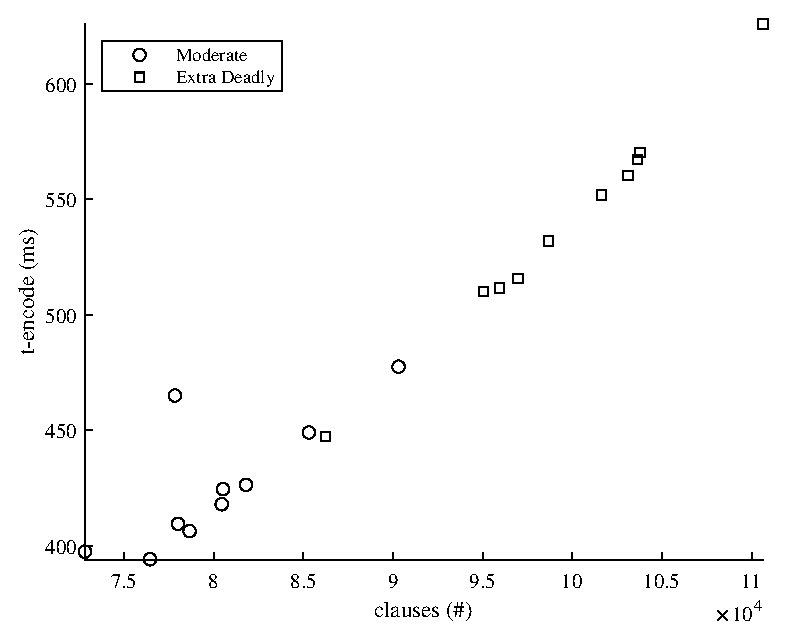
\includegraphics[width = 0.85\textwidth]{Figures/killer_BDD_encode.eps}
    \caption{Encoding time per clause, using Binary Decision Diagrams}
    \label{killerBDDencode}
\end{figure}
\begin{figure}
    \centering
    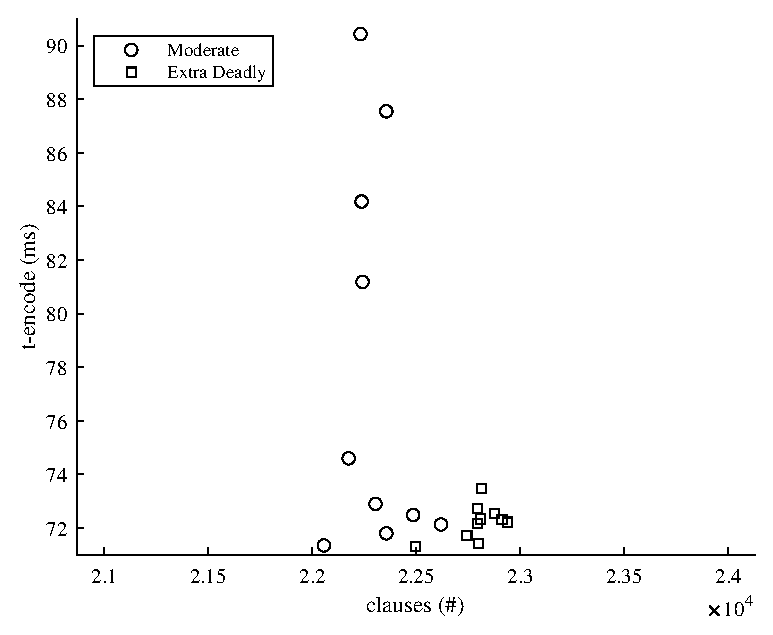
\includegraphics[width = 0.85\textwidth]{Figures/killer_AN_encode.eps}
    \caption{Encoding time per clause, using Adder Networks}
    \label{killerANencode}
\end{figure}

\begin{figure}
    \centering
    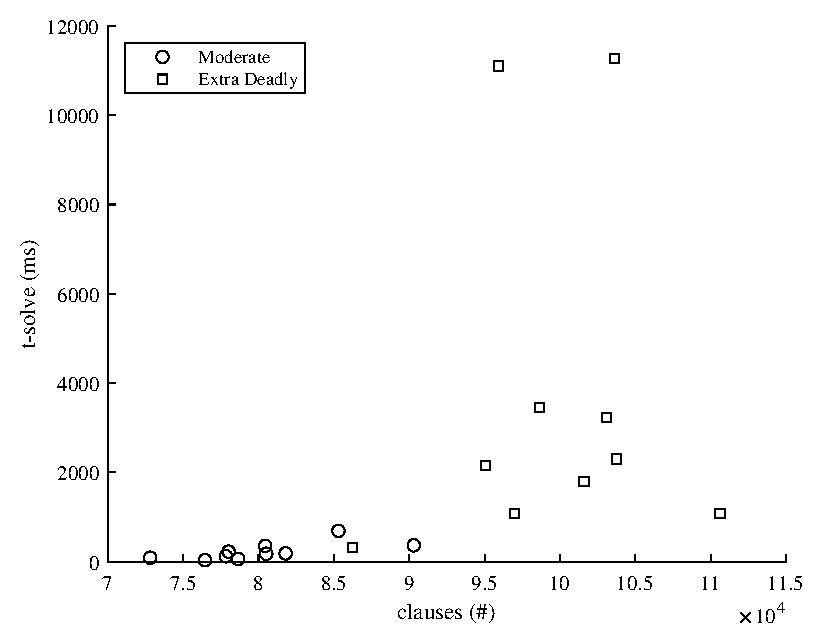
\includegraphics[width = 0.85\textwidth]{Figures/killer_BDD_solve.eps}
    \caption{Solving time per clause, using Binary Decision Diagrams}
    \label{killerBDDsolve}
\end{figure}

\begin{figure}
    \centering
    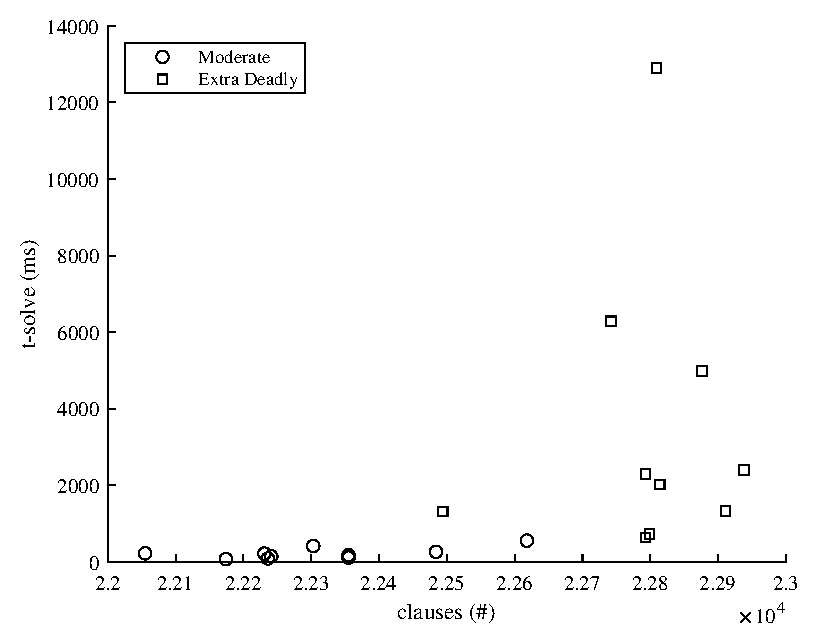
\includegraphics[width = 0.85\textwidth]{Figures/killer_AN_solve.eps}
    \caption{Solving time per clause, using Adder Networks}
    \label{killerANsolve}
\end{figure}

\begin{figure}
    \centering
    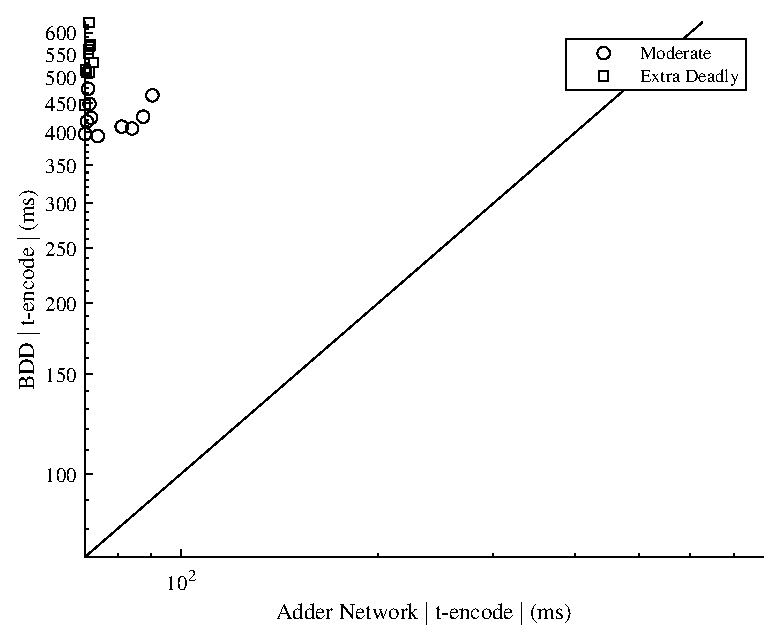
\includegraphics[width = 0.85\textwidth]{Figures/killer_encode_compare.eps}
    \caption{Encoding time comparison, Binary Decision Diagrams vs. Adder Networks}
    \label{killerCompareEncode}
\end{figure}

\begin{figure}
    \centering
    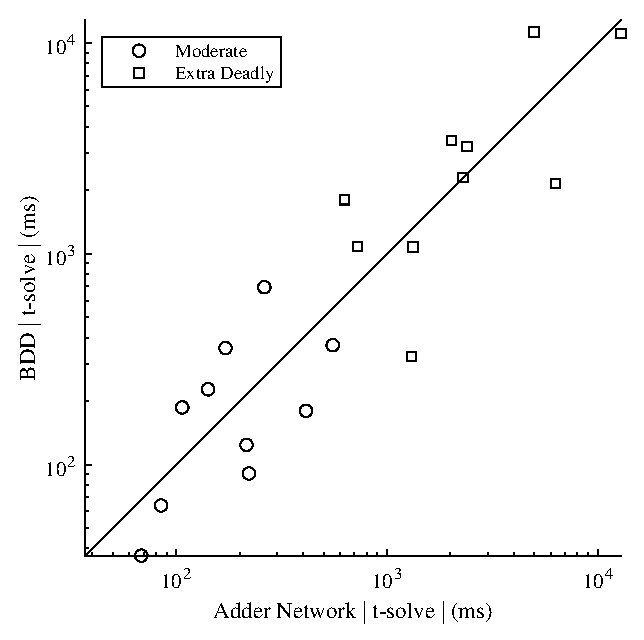
\includegraphics[width = 0.85\textwidth]{Figures/killer_solve_compare.eps}
    \caption{Solving time comparison, Binary Decision Diagrams vs. Adder Networks}
    \label{killerCompareSolve}
\end{figure}
}

{
\renewcommand{\figurename}{Plot}
\begin{figure}
    \centering
    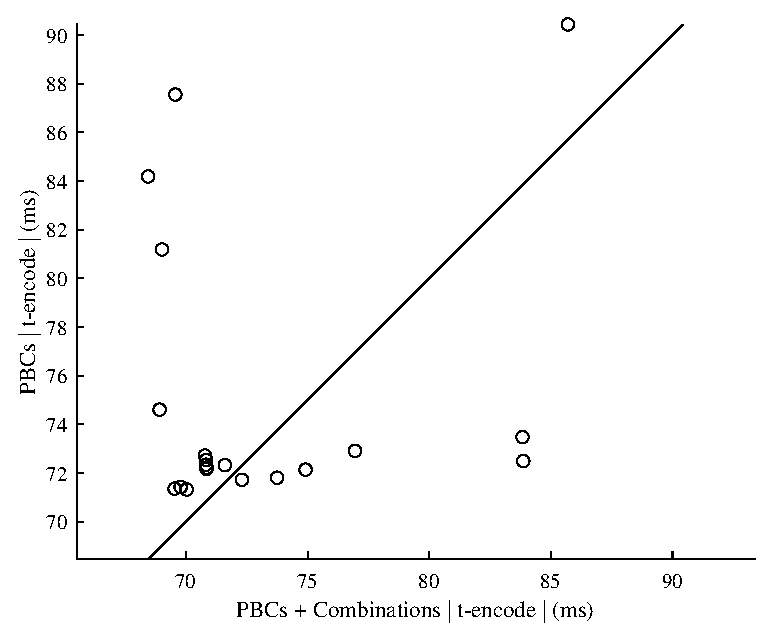
\includegraphics[width = 0.85\textwidth]{Figures/opt_encode_2_1.eps}
    \caption{Encoding time comparison, PBCs vs. PBCs + Combinations}
    \label{opt_encode_2_1}
\end{figure}

\begin{figure}
    \centering
    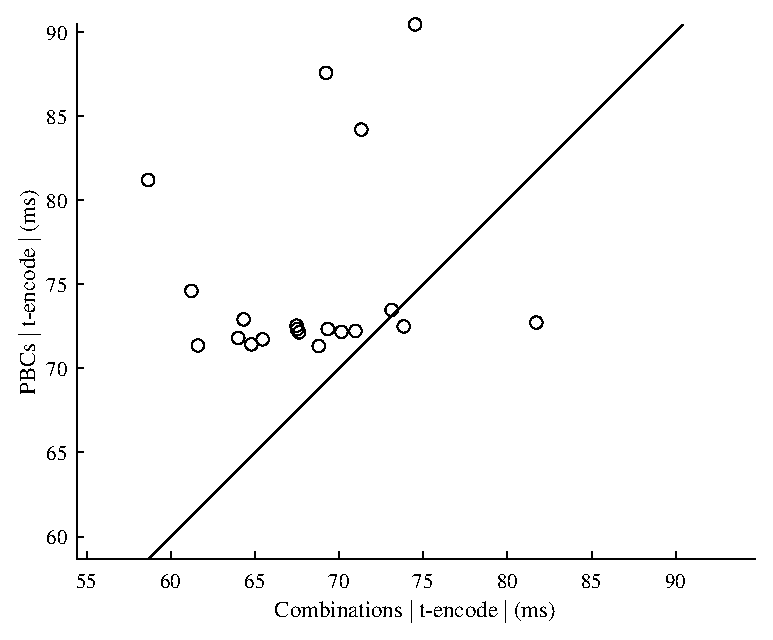
\includegraphics[width = 0.85\textwidth]{Figures/opt_encode_3_1.eps}
    \caption{Encoding time comparison, PBCs vs. Combinations}
    \label{opt_encode_3_1}
\end{figure}

\begin{figure}
    \centering
    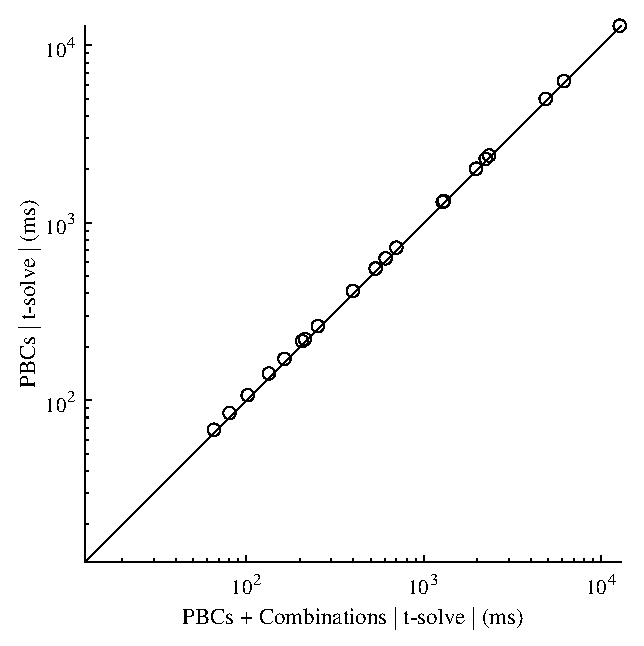
\includegraphics[width = 0.85\textwidth]{Figures/opt_solve_2_1.eps}
    \caption{Solving time comparison, PBCs vs. PBCs + Combinations}
    \label{opt_solve_2_1}
\end{figure}

\begin{figure}
    \centering
    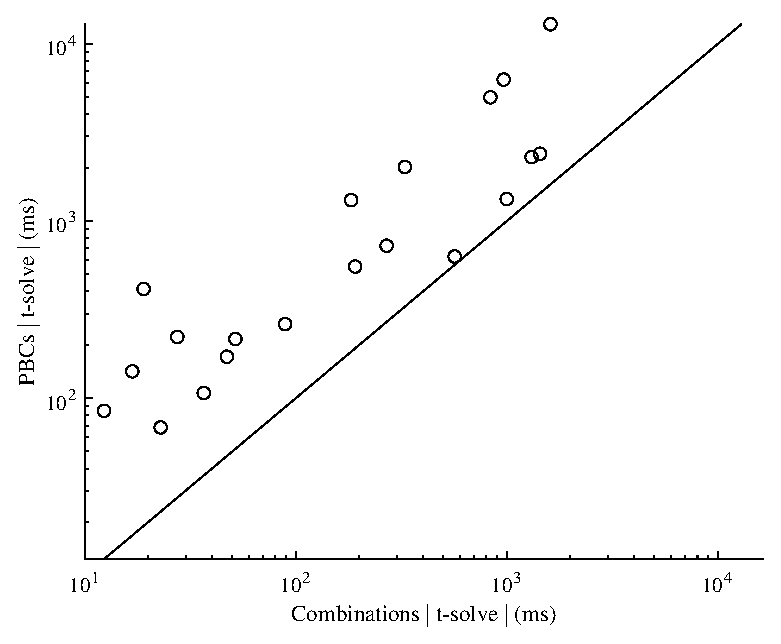
\includegraphics[width = 0.85\textwidth]{Figures/opt_solve_3_1.eps}
    \caption{Solving time comparison, PBCs vs. Combinations}
    \label{opt_solve_3_1}
\end{figure}
}
% !TEX root = ../Thesis.tex
\chapter{Conclusion}
This thesis demonstrated how different variants and rules of Sudoku Puzzles could be encoded as sets of logical clauses. We have seen that in most cases, SAT-solvers can find assignments that satisfy these sets of clauses in a relatively short time. We also found that solving Sudokus is by no means a trivial problem as the number of clauses and the time needed to solve ``Nurikabe Sudoku'' have shown. We have elaborated in detail on how Pseudo Boolean Constraints can be used to encode constraints regarding sums, like in Killer Sudokus or for the Sandwich-Sum rules. Specifically for Killer Sudoku instances, we found that both shown encoding methods Adder Networks and Binary Decision Diagrams (both proposed by \cite{Een2006TranslatingPC}) have comparable performance, but that Adder Networks produce fewer clauses and are encoding the PBCs faster. Additionally, we have shown that encoding Killer Sudokus without PBCs can significantly reduce the time needed to solve them.\\
\\
In future work, the proposed encoding methods for Sudoku rules could help to craft new puzzle instances of exotic Variants like ``9 Marks The Spot'' or ``The Miracle Thermo''. Further, we came across multiple engaging questions for which we only estimated an answer or gave an upper bound, like what is the highest possible number of islands in ``Nurikabe Sudoku" or how long can a hidden path in ``9 Marks The Spot'' be at maximum. Also teasing: CTCGH \cite{CrackingTheCryptic2021} contains many more Sudoku variants which could be analysed and encoded for SAT-Solvers.\\
\\
During our work, we only used a limited test set of puzzle instances, which all had to be rewritten by hand into a format our program could understand. In general, there seem to be no common test sets for non-original Sudoku Variants like Killer Sudoku, which may also has to do with the lack of a common file format that could be used to share more exotic Puzzle variants. To facilitate future work, it would be desirable to agree on a standard file format specifically tailored for Sudokus. This would allow the puzzle and research community to build an openly available and directly usable database of Sudoku Puzzles, which would make the testing and analysis of new encoding and solving algorithms more reliable.
%\input{./Chapters/Chapter7}
%% ----------------------------------------------------------------
\thesisappendix
\thesisbib
\begin{appendices}
	%\input{./Back/AppendixA} 
\end{appendices}
%% ----------------------------------------------------------------
\thesisback
\iflanguage{english}
  {\includepdf{./Back/wissensch_Redlichkeit_E_Aug_21.pdf}}
  {\includepdf{./Back/wissensch_Redlichkeit_D_Aug_21.pdf}}
%% ----------------------------------------------------------------
\end{document}
%% ----------------------------------------------------------------
